\subsection{P0D Tracking and Matching Efficiency}
\label{sec:Systematics_Efficiency}

The efficiency of reconstruction, and the differences between Monte Carlo and data efficiencies, are the first source of systematic uncertainty studied for the CC Inclusive selection. There are several steps involved in reconstructing the final candidate muon track as described in previous sections. In this section, we use a `FGD Cosmic' sample to  investigate the reconstruction and matching efficiencies of our analysis. Cosmics provide a sample independent of the physics we are probing, and are an excellent unbiased sample to use to evaluate the efficiency systematic. However, as Cosmics do not have the same bunched timing structure as our beam events, we also used as independent sample of sand muons from Production 4 to cross check our results. The results of the cross check are summarized in Section \ref{sec:Appendix_sandmuoneff}. Efficiencies extracted from Production 4 cosmics and sand muons and Production 5 cosmics agree well.
Sand Muons are generated by beam neutrinos interacting with material outside the off-axis near detector and so have a timing strucutre that mimics that of beam events. 
These two 'sideband' samples together provide a robust method for evaluating the matching and reconstruction efficiency systematic. Finally, we also performed a hand-scan of beam events in Production 4 reconstruction files to identify and quantify any reconstruction issues missed with the FGD cosmics and sand muon samples.\\

We use a simple method to examine the efficiency of our matching algorithm for tracks that deposit energy in the \p0d, enter the Tracker and are reconstructed by the Tracker reconstruction package. We simultaneously determine how often P0D reconstruction successfully fits a track and how often we succesfully match this track with a Tracker reconstructed track. First, we pre-select a sample of quality tracks reconstructed in TPC1 that point squarely into the 
\p0d. We then attempt to pair each of these tracks to a \p0d reconstructed track. The ratio of the number of matched pairs found to the number of quality TPC1 tracks yields the 'matching efficiency'. Though this estimate is not necessarily the absolute efficiency, given that monte carlo simulates data well to the first order, the observed difference between the monte carlo efficiency and the data efficiency gives us the systematic due to reconstruction and matching.

This definition folds in the \p0d's intrinsic, lower level reconstruction efficiencies (i.e. hit finding, \p0d-only tracking, etc.) as well as matching and recombination efficiencies from the matching algorithm. However, as we use reconstructed tracks in the ND280 Tracker as a baseline, we do not account for the Tracker tracking efficiency with this strategy. We determine the systematic uncertainty from the Tracker efficiency separately in a later section.\\

\subsubsection{Cosmics Sample}
\label{sec:CosmicsEfficiency}

Using the `FGD Cosmics' sample, we extract the matching efficiency as defined above. The following determine the denominator and numerator. Note that for the numerator of the efficiency, the cuts closely mimic those used in Sections \ref{sec:EventReconstruction} and \ref{sec:InclusiveAnalysis} to select muon candidates. Also, the pre-selection cuts are slightly different between the Cosmics sample as opposed to the Sand Muon sample. The necessity for this difference is discussed later.\\

Pre-Selection Cuts (Denominator):

\begin{enumerate}
\item There must be a Tracker reconstructed track in the event
\item The Tracker track must be reconstructed as beginning at the upstream face of the first TPC (Z \(<\) -750 mm)
\item The TPC must measure a momentum of at least 250 MeV
\item Project the Tracker track linearly backwards into the \p0d. The projection is made to the Z = -1100 mm plane, and then just the XY fiducial cut is applied to the projected point.
\item The Tracker track has \(>\) 18 reconstruction nodes
\item The Tracker track has a `corrected time' stamp between -4800ns and -4400ns. The time correction allows us to find the tracker time in relation to the \p0d electronics. The time cut is placed 80ns from the edge of the 480ns-wide \p0d integration window. This is the window where the \p0d electronics are capable of properly reconstructing hits. For a more detailed discussion of the timing cut, please refer to Appendix section \ref{sec:Appendix_p0delec.}
%\item There are at least 3 `good \p0d hits'. A `good hit' is defined as a 7 p.e. or greater \p0d hit which is found within a certain region of the \p0d and with a certain time. The region we search is a cone with opening angle of 30 degrees and length of 250mm. The time is required to be 80ns from the edge of the \p0d integration window. We make this cut to assure that no noise hits or hits with invalid timing due to known electronics design, are contaminating our pre-selection. For a more detailed discussion of the timing cut, please refer to Appendix section \ref{sec:Appendix_p0delec.}
\end{enumerate}

Matching Cuts (Numerator):
\begin{enumerate}
\item All pre-selection cuts are made as above
\item P0D Vertex must be reconstructed by TP0DPairwiseVertexPID algorithm and the track must be a constituent of this vertex
\item P0D Track must be exiting as defined by the last node having a Z position $>$ -1016 mm
\item P0D Track must be 3D as defined by cutting on track position variance
%\item Correct for alignment (x = 7 mm, y = 26 mm) in data only. 
Evaluate $\Delta R$, $\Delta \sin \theta$  and $\Delta T$ between the p0d track projection and tracker track as before. Apply the following cuts: $\Delta R$ \(<\) 86mm, $\Delta \sin \theta$ \(<\) .76, $\Delta T$ \(<\) 100 ns.
\end{enumerate}

The number of tracks passing the numerator cuts divided by the number passing the denominator cuts yields the efficiency. Figures \ref{fig:eff_dR} and \ref{fig:eff_dSdT} show the matching parameter distributions for $\Delta R$, $\Delta X$, $\Delta Y$, $\sin \Delta \theta$ and $\Delta T$. 
The $\Delta Y$ distribution does not agree very well and causes some disagreement in the $\Delta R$ distribution as well. This discrepancy has been isolated to a difference between forward going and backwards going cosmics tracks as determined by the Tracker reconstruction. Figure \ref{fig:dY} shows the $\Delta Y$ residuals separated by forward and backwards going tracks for FGD Cosmics in Data and MC. Note that in MC, the two different directions have a small shift in the central value of the residual. However, in Data, the shift is much greater. Using Production 4 to demonstrate the effect, we have fit gaussians to all of the residuals. The results are shown in Table \ref{tab:FitdY}. The root cause of this effect is a difference in the geometry used for reconstruction and the geometry of the `as built' detector. A much more detailed investigation and the results are discussed in the Appendix in Section \ref{sec:Appendix_align}. Finally, note that since the $\Delta R$ agreement between Data and MC for the Cosmics sample is actually worse than the Beam events, the evaluated uncertainty should be conservative. 
Similarly, though the timing distribution does not agree as well as the others, the timing cut is large enough to account for the overall shift. 


\begin{figure}
\centering
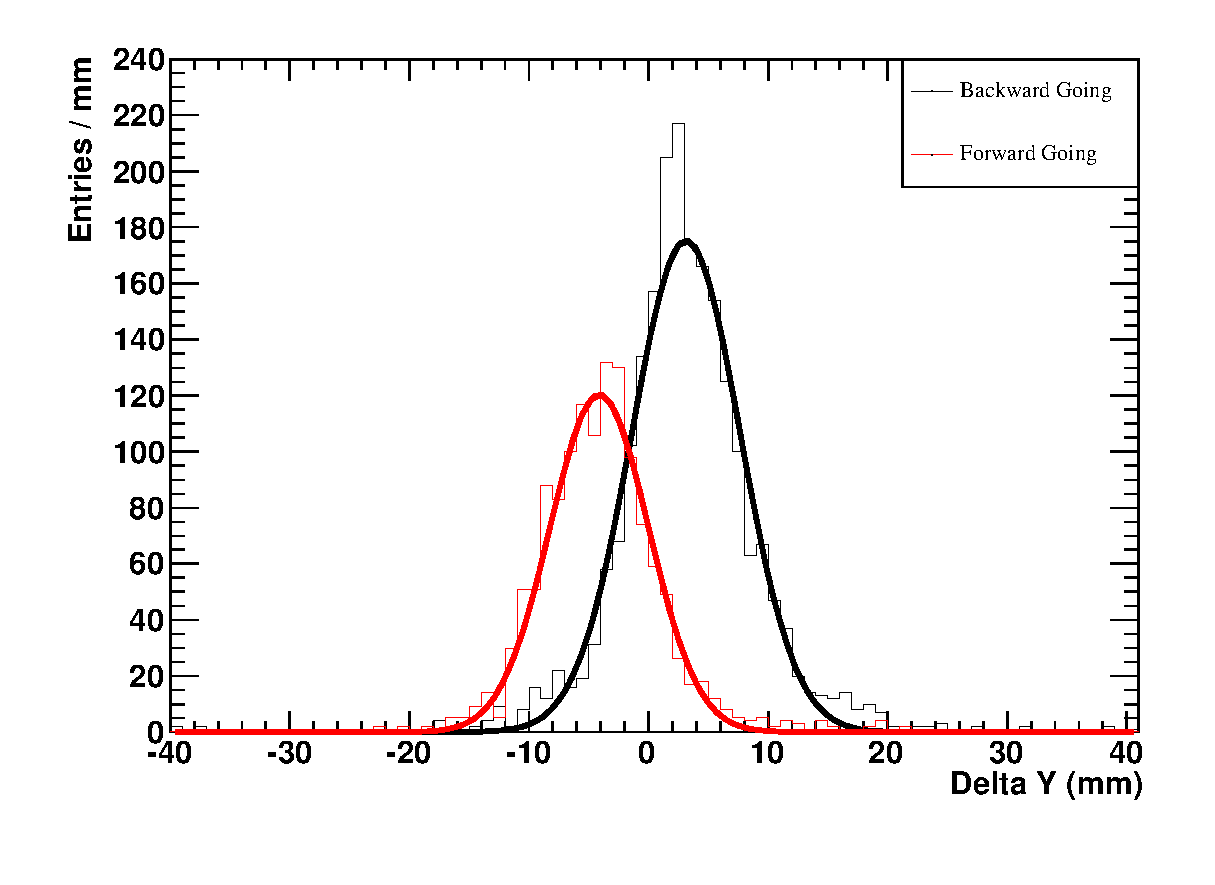
\includegraphics[width=2.5in]{Figures/Systematics/MatchingEfficiency/datadY.eps}
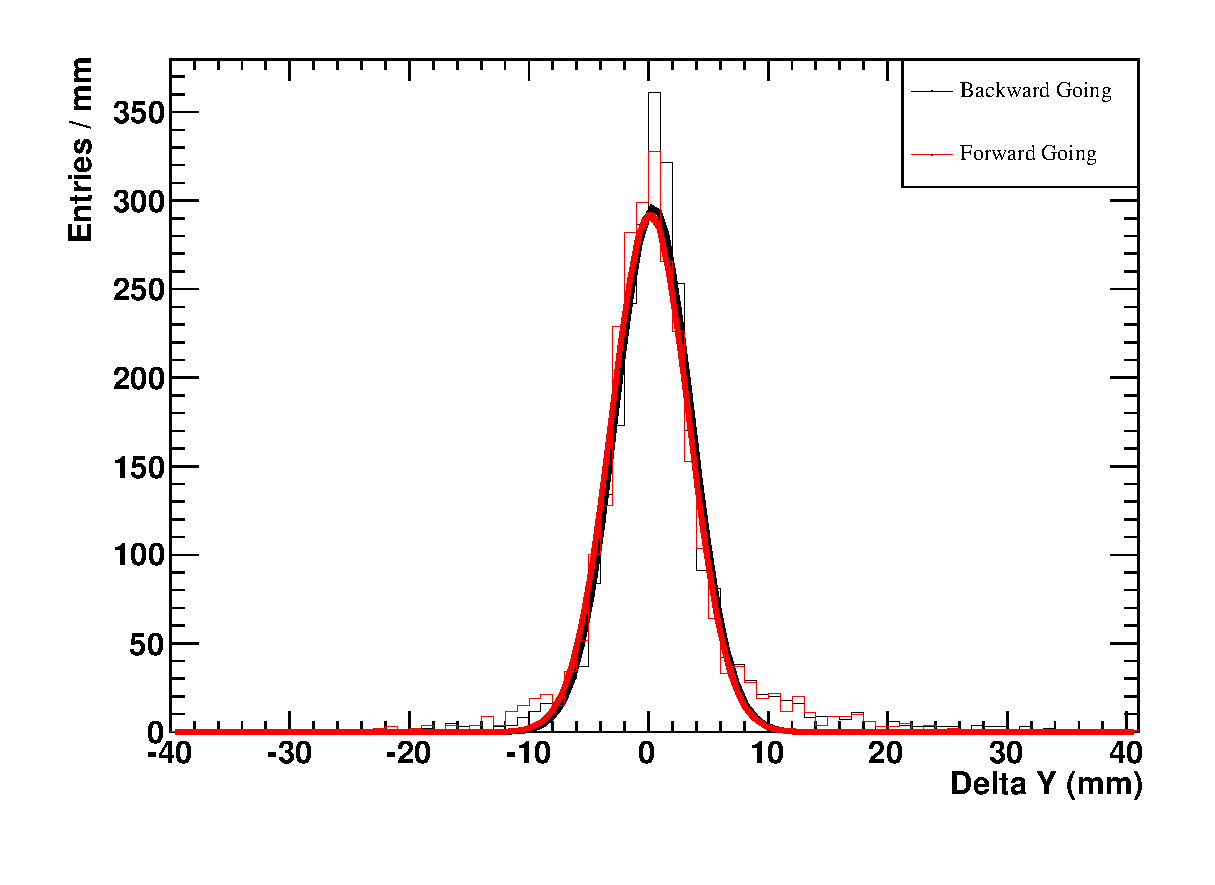
\includegraphics[width=2.5in]{Figures/Systematics/MatchingEfficiency/mcdY.eps}
\caption{
Matching Parameter $\Delta$ Y for Production 4 FGD cosmics in Data and MC split into forward and backward going tracks. Gaussian fits have been overlayed. The left plot shows the shift in the residual in Data cosmics when comparing forward (red) and backward (black) tracks. The right plot shows that in MC we do not see such a shift between forward (red) and backward (black) tracks.
}
\label{fig:dY}
\end{figure}

\begin{table}
\centering
\begin{tabular}{lccc}\toprule\midrule
Type and Dir. &  Mean & Sigma & $\chi^2$/NDOF \\ \midrule
Data Forward & $-4.1\pm 0.1$ & $4.1\pm 0.1$ & $100.0/48$  \\
\midrule
Data Backward & $3.1\pm 0.1$ & $4.5\pm 0.1$ & $155.2/58$ \\
\midrule
MC Forward & $0.1\pm 0.1$ & $3.2\pm 0.1$ & $255.1/51$ \\
\midrule
MC Backward & $0.5\pm 0.1$ & $3.2\pm 0.1$ & $263.2/59$ \\
\bottomrule
\end{tabular}
\caption{Gaussian fit results and fit error of $\Delta Y$ for 10000 Production 4 FGD Cosmics in Data and MC. The results are divided into backwards and forward going cosmics as determined by the Tracker reconstruction.}
\label{tab:FitdY}
\end{table}

\begin{figure}
\centering
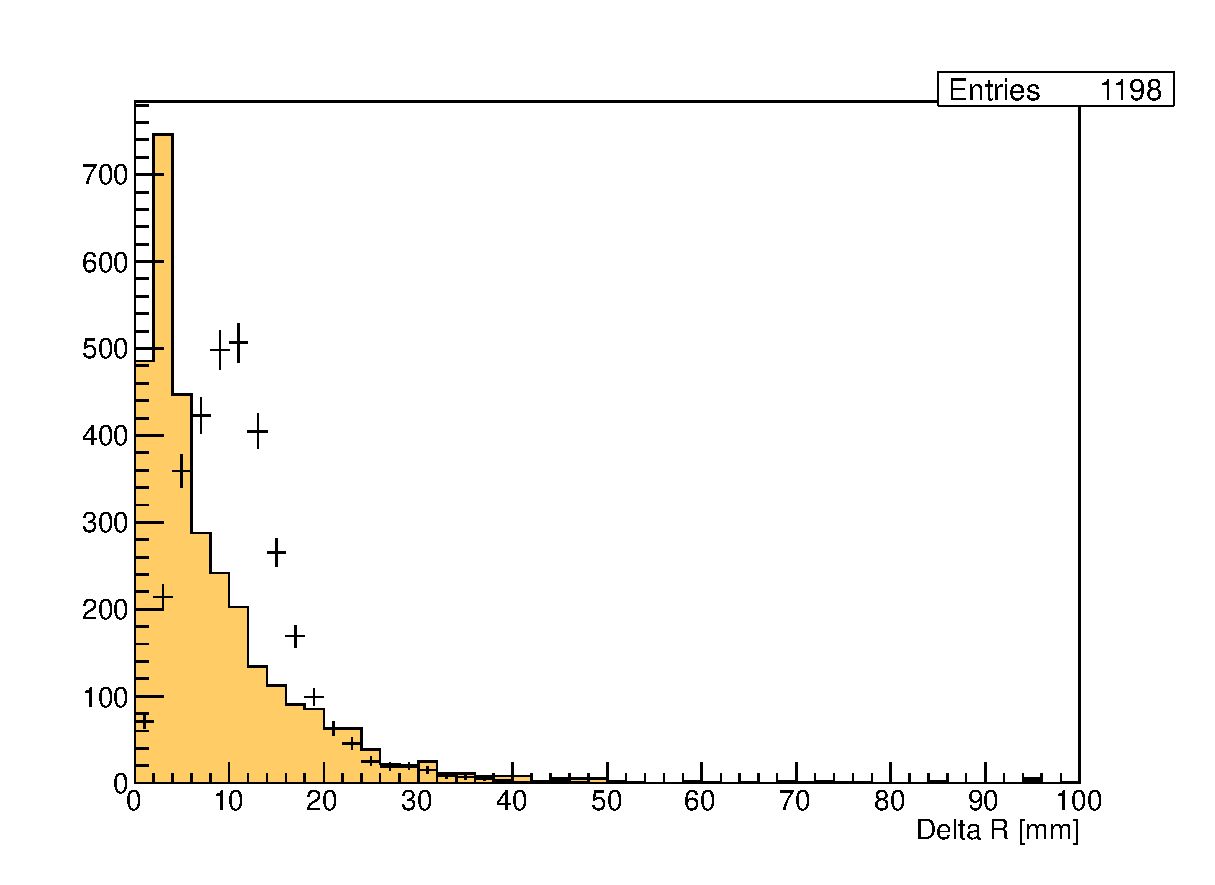
\includegraphics[width=2in]{Figures/Systematics/MatchingEfficiency/dRcosmics.eps}
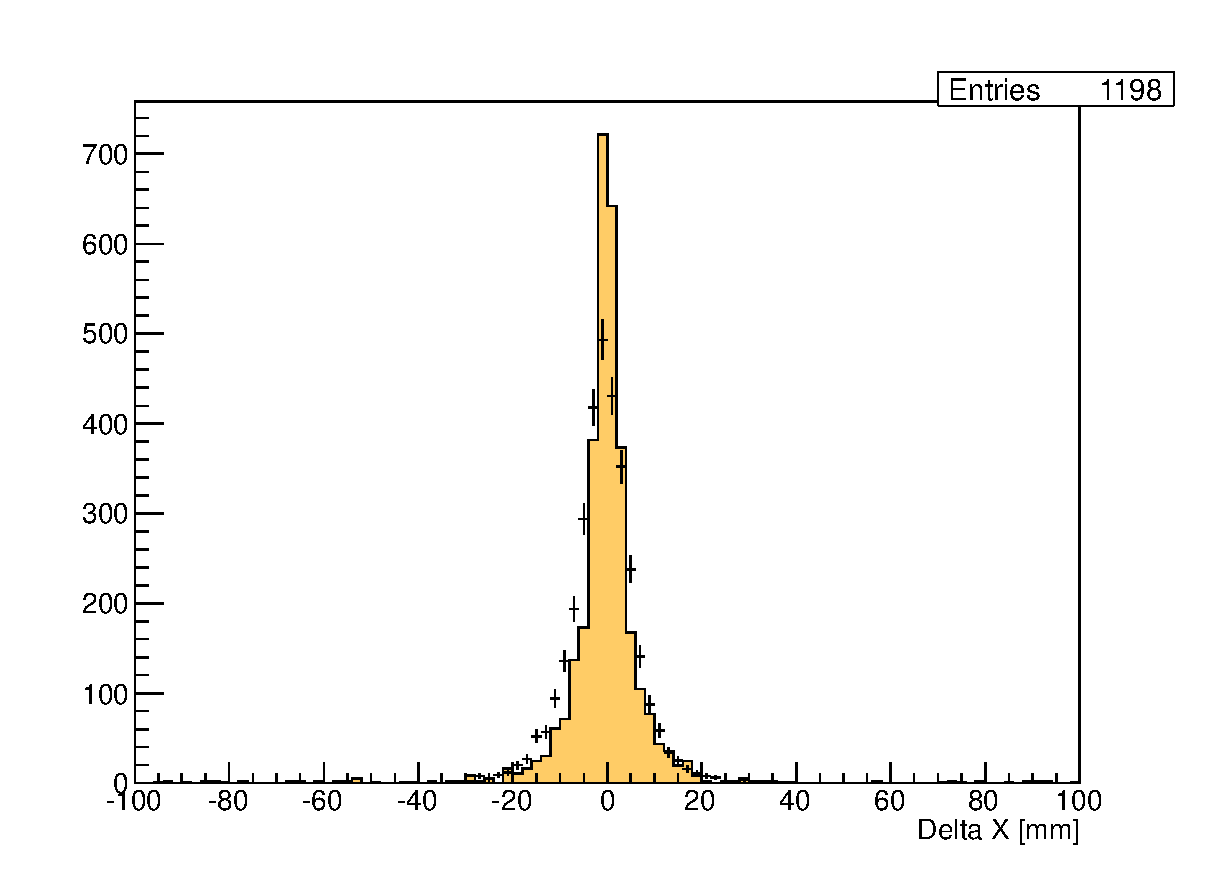
\includegraphics[width=2in]{Figures/Systematics/MatchingEfficiency/dXcosmics.eps}
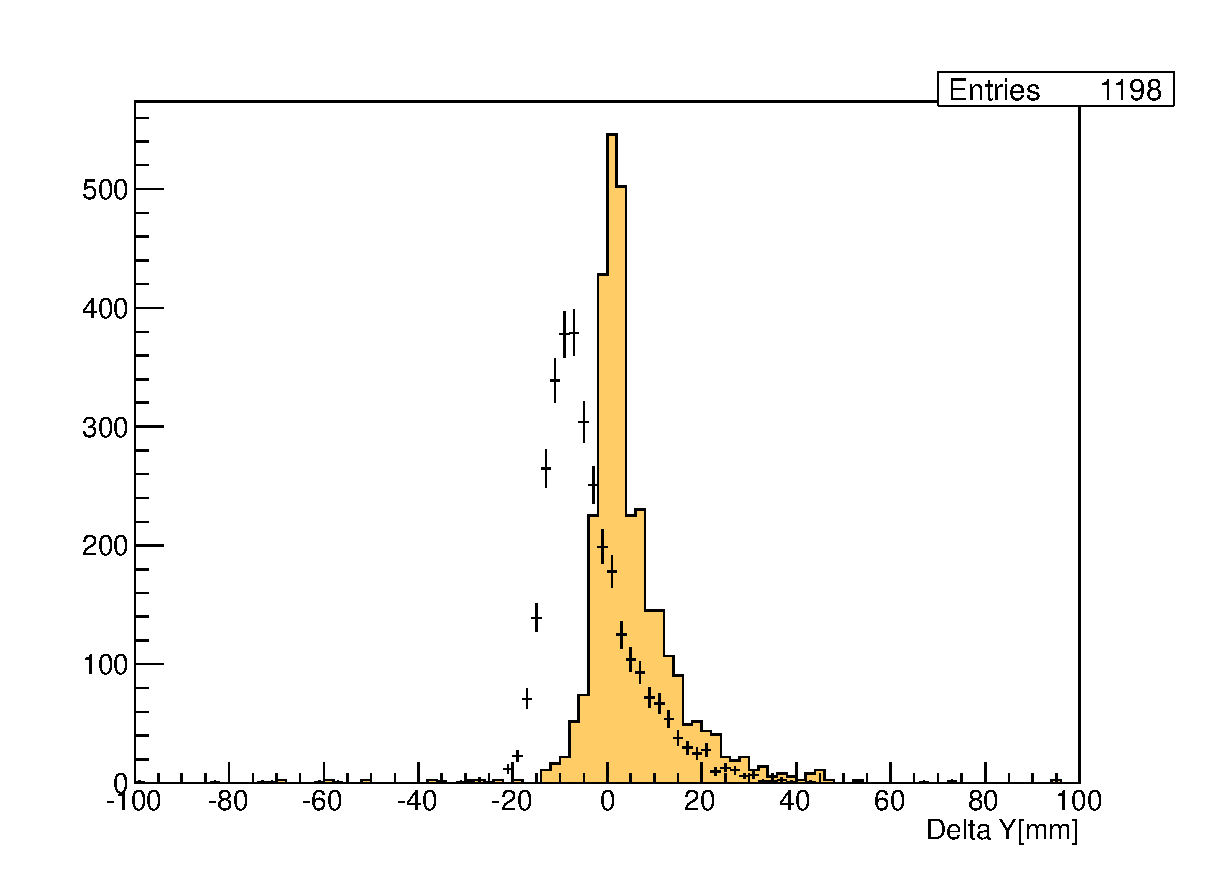
\includegraphics[width=2in]{Figures/Systematics/MatchingEfficiency/dYcosmics.eps} 
\caption{
Matching Parameters $\Delta$ R, $\Delta$ X, and $\Delta$ Y for cosmics. The matching cut is applied only on $\Delta$ R. Black dots with error bars denote data while the orange fill is monte carlo. We note that the difference in shape in $\Delta$ R distributions is due to a shape difference in $\Delta$ Y between data and MC.
}
\label{fig:eff_dR}
\end{figure}

\begin{figure}
\centering
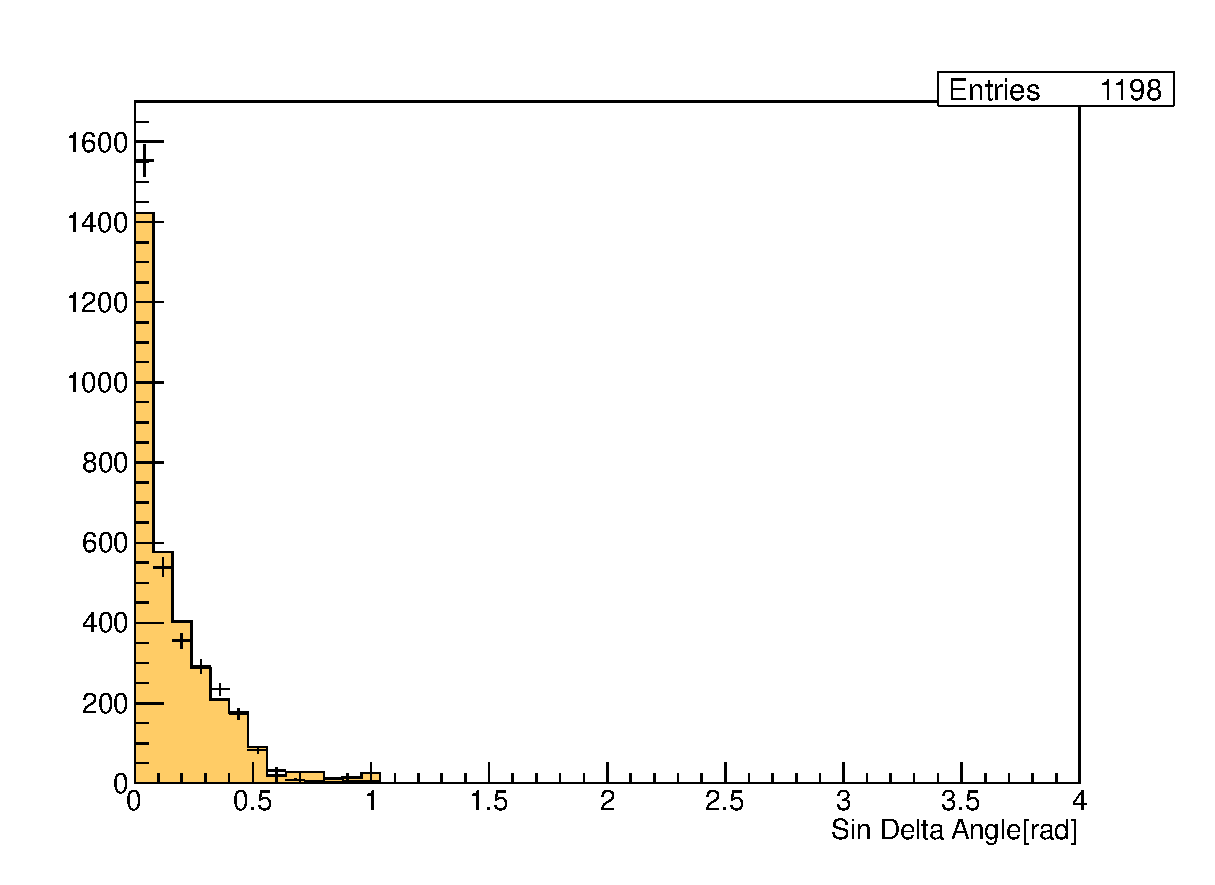
\includegraphics[width=2.5in]{Figures/Systematics/MatchingEfficiency/dScosmics.eps}
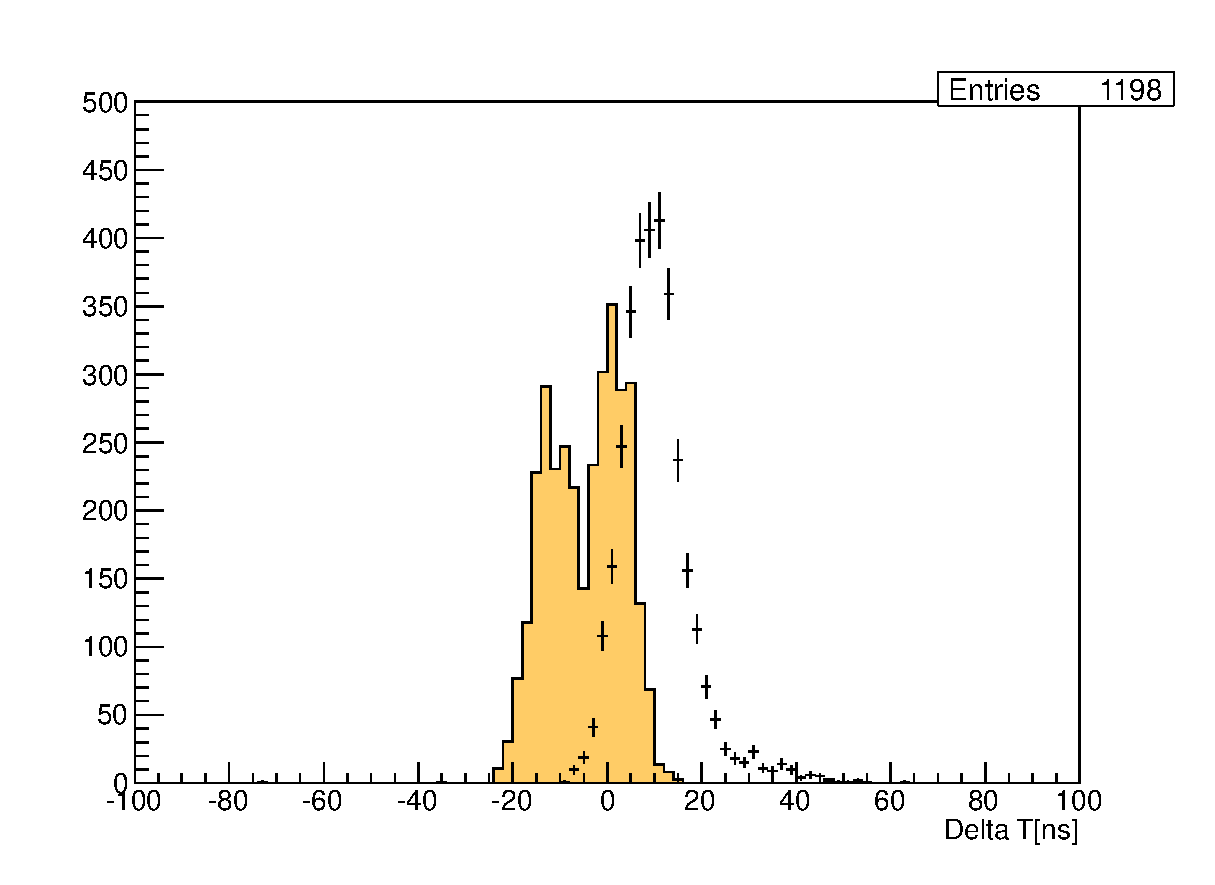
\includegraphics[width=2.5in]{Figures/Systematics/MatchingEfficiency/dTcosmics.eps}
\caption{Cosmics matching efficiency parameters \(\sin \theta\) and \(\Delta T\). The difference in \(\Delta T\) is not understood, but the cut is placed wide enough to be insensitive to the overall shift.}
\label{fig:eff_dSdT}
\end{figure}

\begin{figure}
\centering
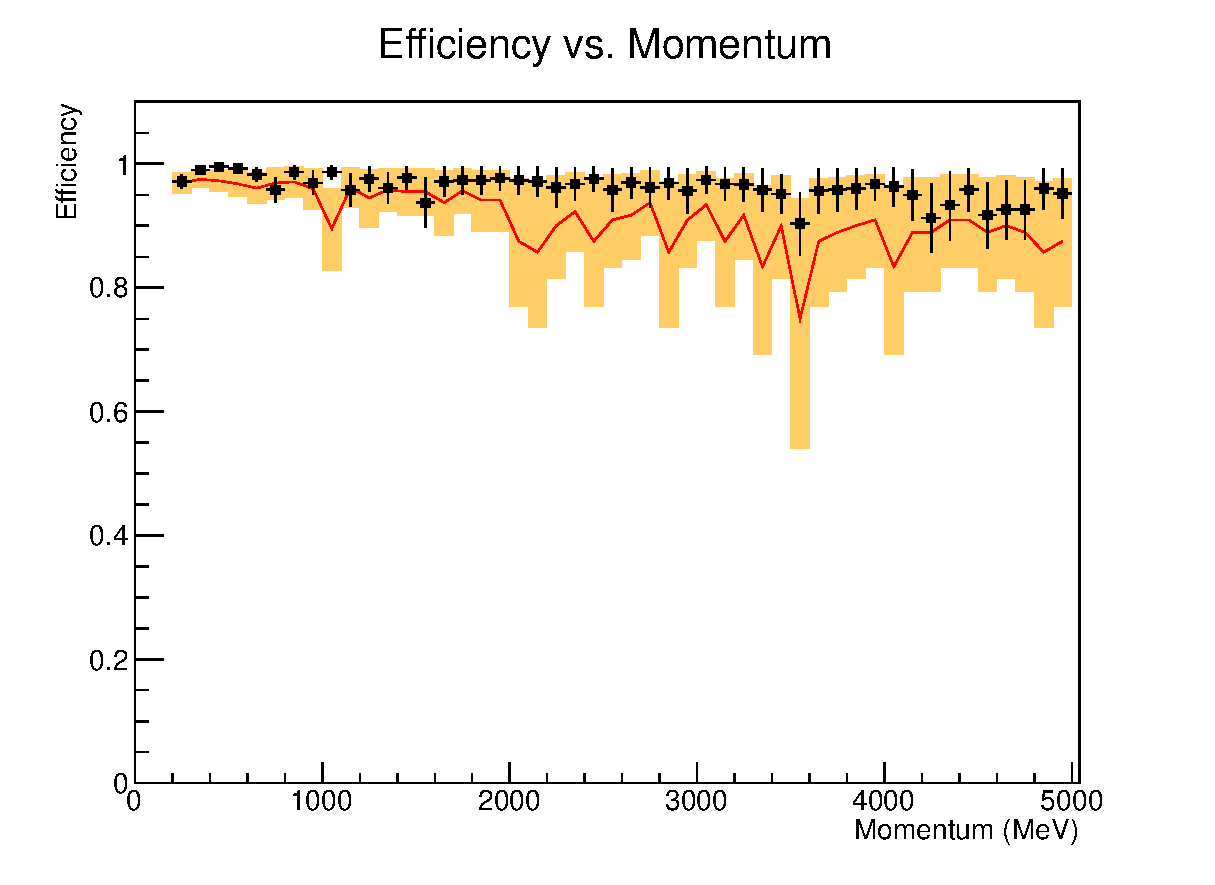
\includegraphics[width=3in]{Figures/Systematics/MatchingEfficiency/Eff_vs_Momentum.eps}
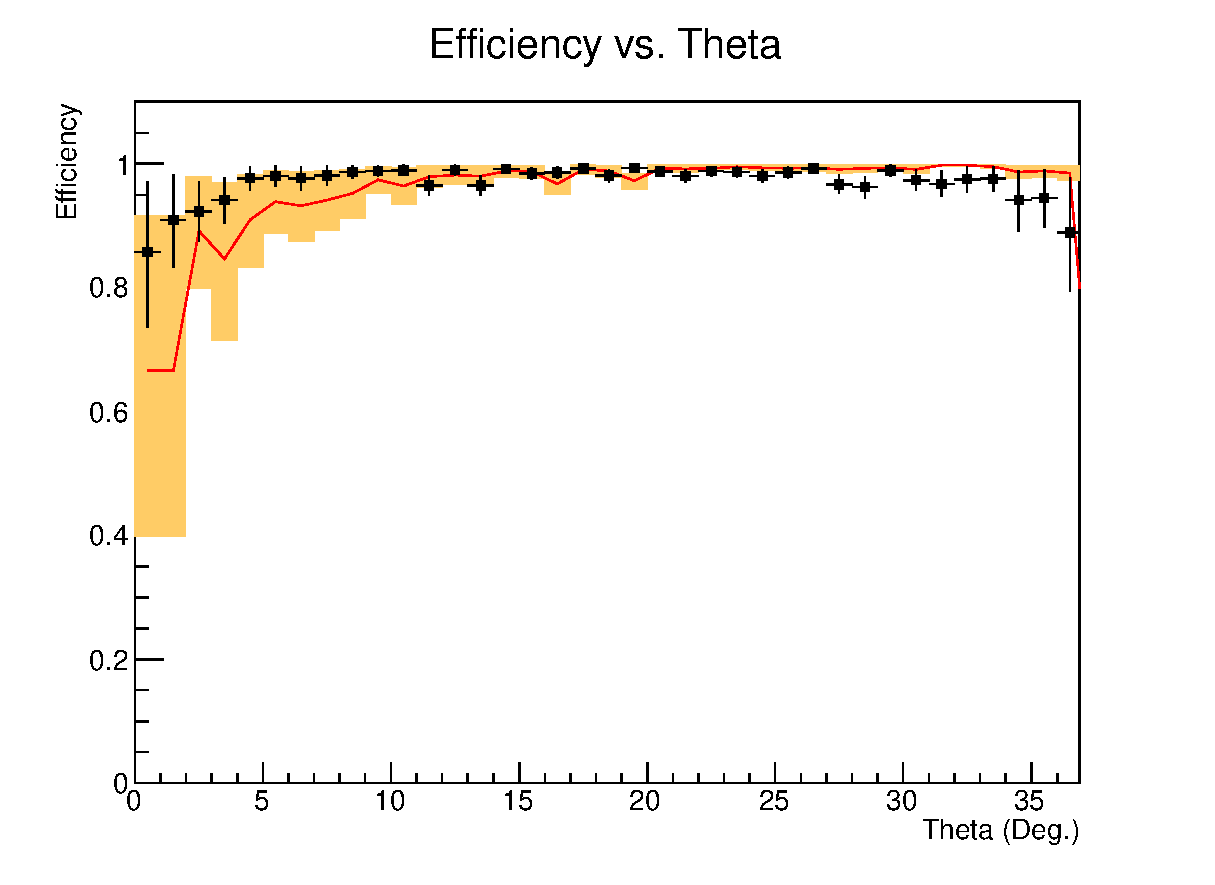
\includegraphics[width=3in]{Figures/Systematics/MatchingEfficiency/Eff_vs_Theta.eps}
\caption{Cosmics efficiencies as a function of Momentum and \(\theta\). Black dots are data and red line is the MC. The orange fill shows the error on the MC. We note that the data and MC efficiencies track each other as a function of both kinematic variables.}
\label{fig:eff_ND}
\end{figure}

Figure \ref{fig:eff_ND} then shows the final efficiency values for data and MC as a function of muon momentum and $\theta$. Note that in Figure \ref{fig:eff_ND}, the statistical errors are calculated using a probability distribution function derived with a bayesian approach. The derivation of the PDF can be found in a paper by M. Paterno~\cite{bayes} and is implemented in ROOT under the TEfficiency class. The central values in Figure \ref{fig:eff_ND} are then the mean of the PDF (as opposed to the median). The statistical error for the integrated ratio is calculated more simply by approximating the efficiency as a binomial distribution. The efficiencies from the FGD cosmics sample are $99.08\%\pm 0.16\%$ for Data and $99.22\%\pm 0.24\%$ for MC.

\subsubsection{Reconstruction Failures in Beam Events}

We also performed a search for unclassified reconstruction failures in beam events in Production 4 to account for any possible systematic effect missed by the FGD cosmics and sand muons study. Similar to the method in Section \ref{sec:CosmicsEfficiency}, beam events with one or two quality Tracker tracks pointing directly into the P0D were pre-selected. As the Data has a large number of sand muons present, we also added a cut to veto these events. If more than two above-noise hits were found in the outer edges of the \p0d coincident in time with the TPC1 track, we tag the event as a sand muon and exclude it. Of the remaining events, we filtered out those where the matching algorithm failed to find a suitable \p0d track to match with the Tracker piece. Finally, the filtered events were examined by hand using an event plotting software (plot-event.exe) to identify any potential reconstruction pathologies previously missed.

When hand scanning filtered events, we founds several modes of failure, many of which were expected. For example, events which had short or partially reconstructed tracks in the downstream end of the \p0d as well events with no \p0d constituent were missed by the matching algorithm for obvious reasons. Furthermore, some DIS-like events had large clusters of energy deposits in the \p0d and were difficult to separate properly into tracks. These were also missed by the matching algorithm as expected. However, there were three classes of failure which, by eye, looked as if they should have been successfully matched. These we examined more closely.

First, we found events with multiple clean tracks passing into TPC1 which were missed by our algorithm. Further study showed this failure mode existed both in Data and MC and was an expected effect. In Appendix Section \ref{sec:Appendix_ambig} we explain how a reconstruction amibiguity (due to design) causes a small portion of multi track events to fail the matching algorithm. Second, we found another class of failed events where the \p0d and Tracker tracks were well matched spatially, but separated widely in time ($\Delta T$ failure). Finally, the last failure mode were events where the \p0d and Tracker tracks were mismatched in the XZ projection, a symptom of incorrect T0 extraction at the TPC1 reconstruction stage. An incorrect T0 calculation creates an offset in the TPC drift direction (XZ). Please see the ND280 reconstruction technical note \cite{tn72} for greater detail. Figure \ref{fig:mismatchexamples} shows examples of the $\Delta T$ and $T0$ failure modes.

\begin{figure}[h]
  \centering
  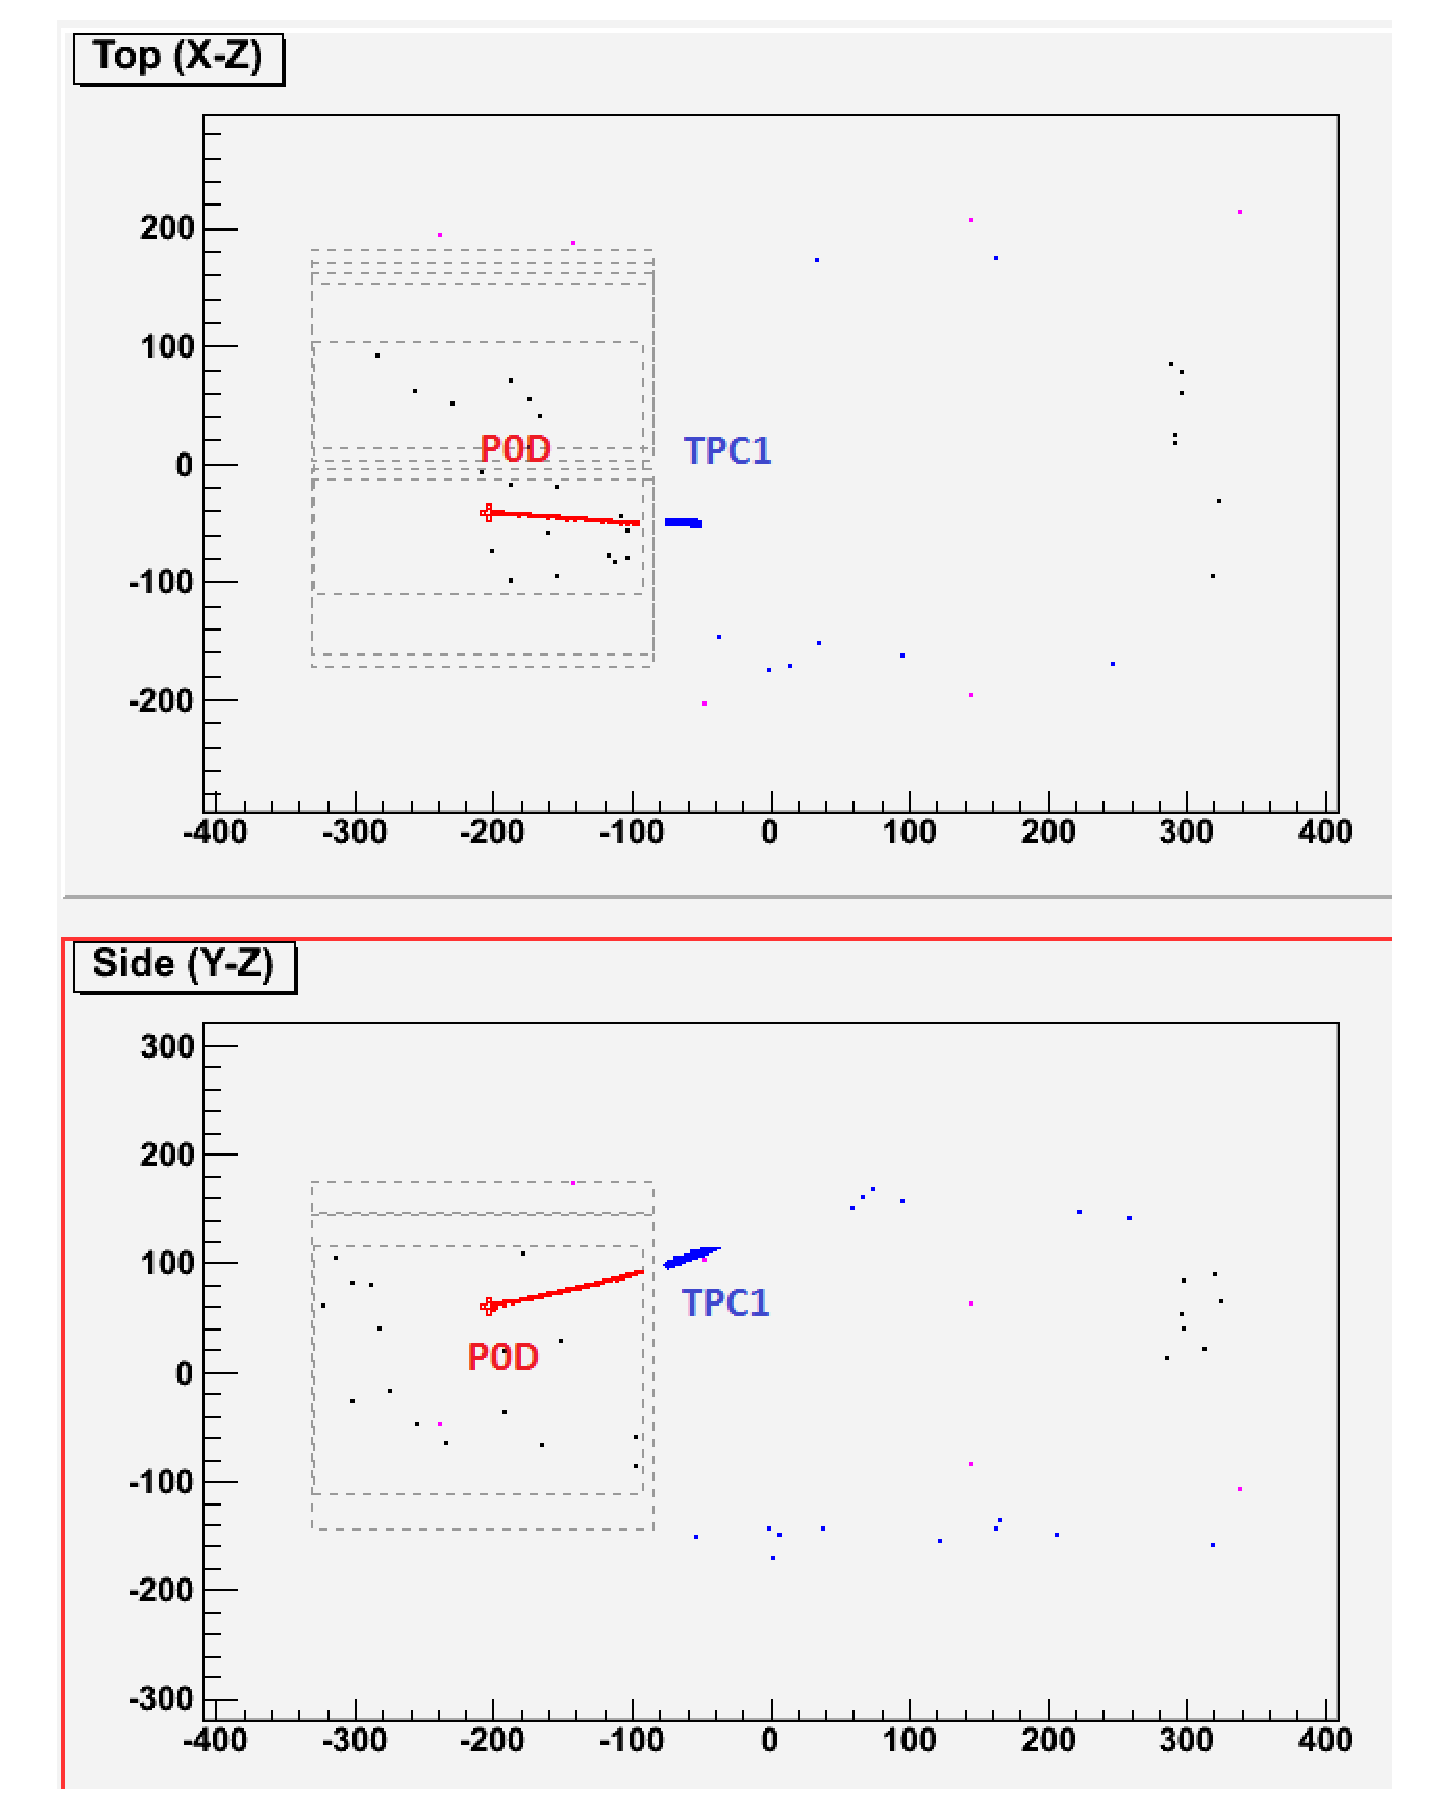
\includegraphics[width=3in]{Figures/delltaTmismatch.eps}
  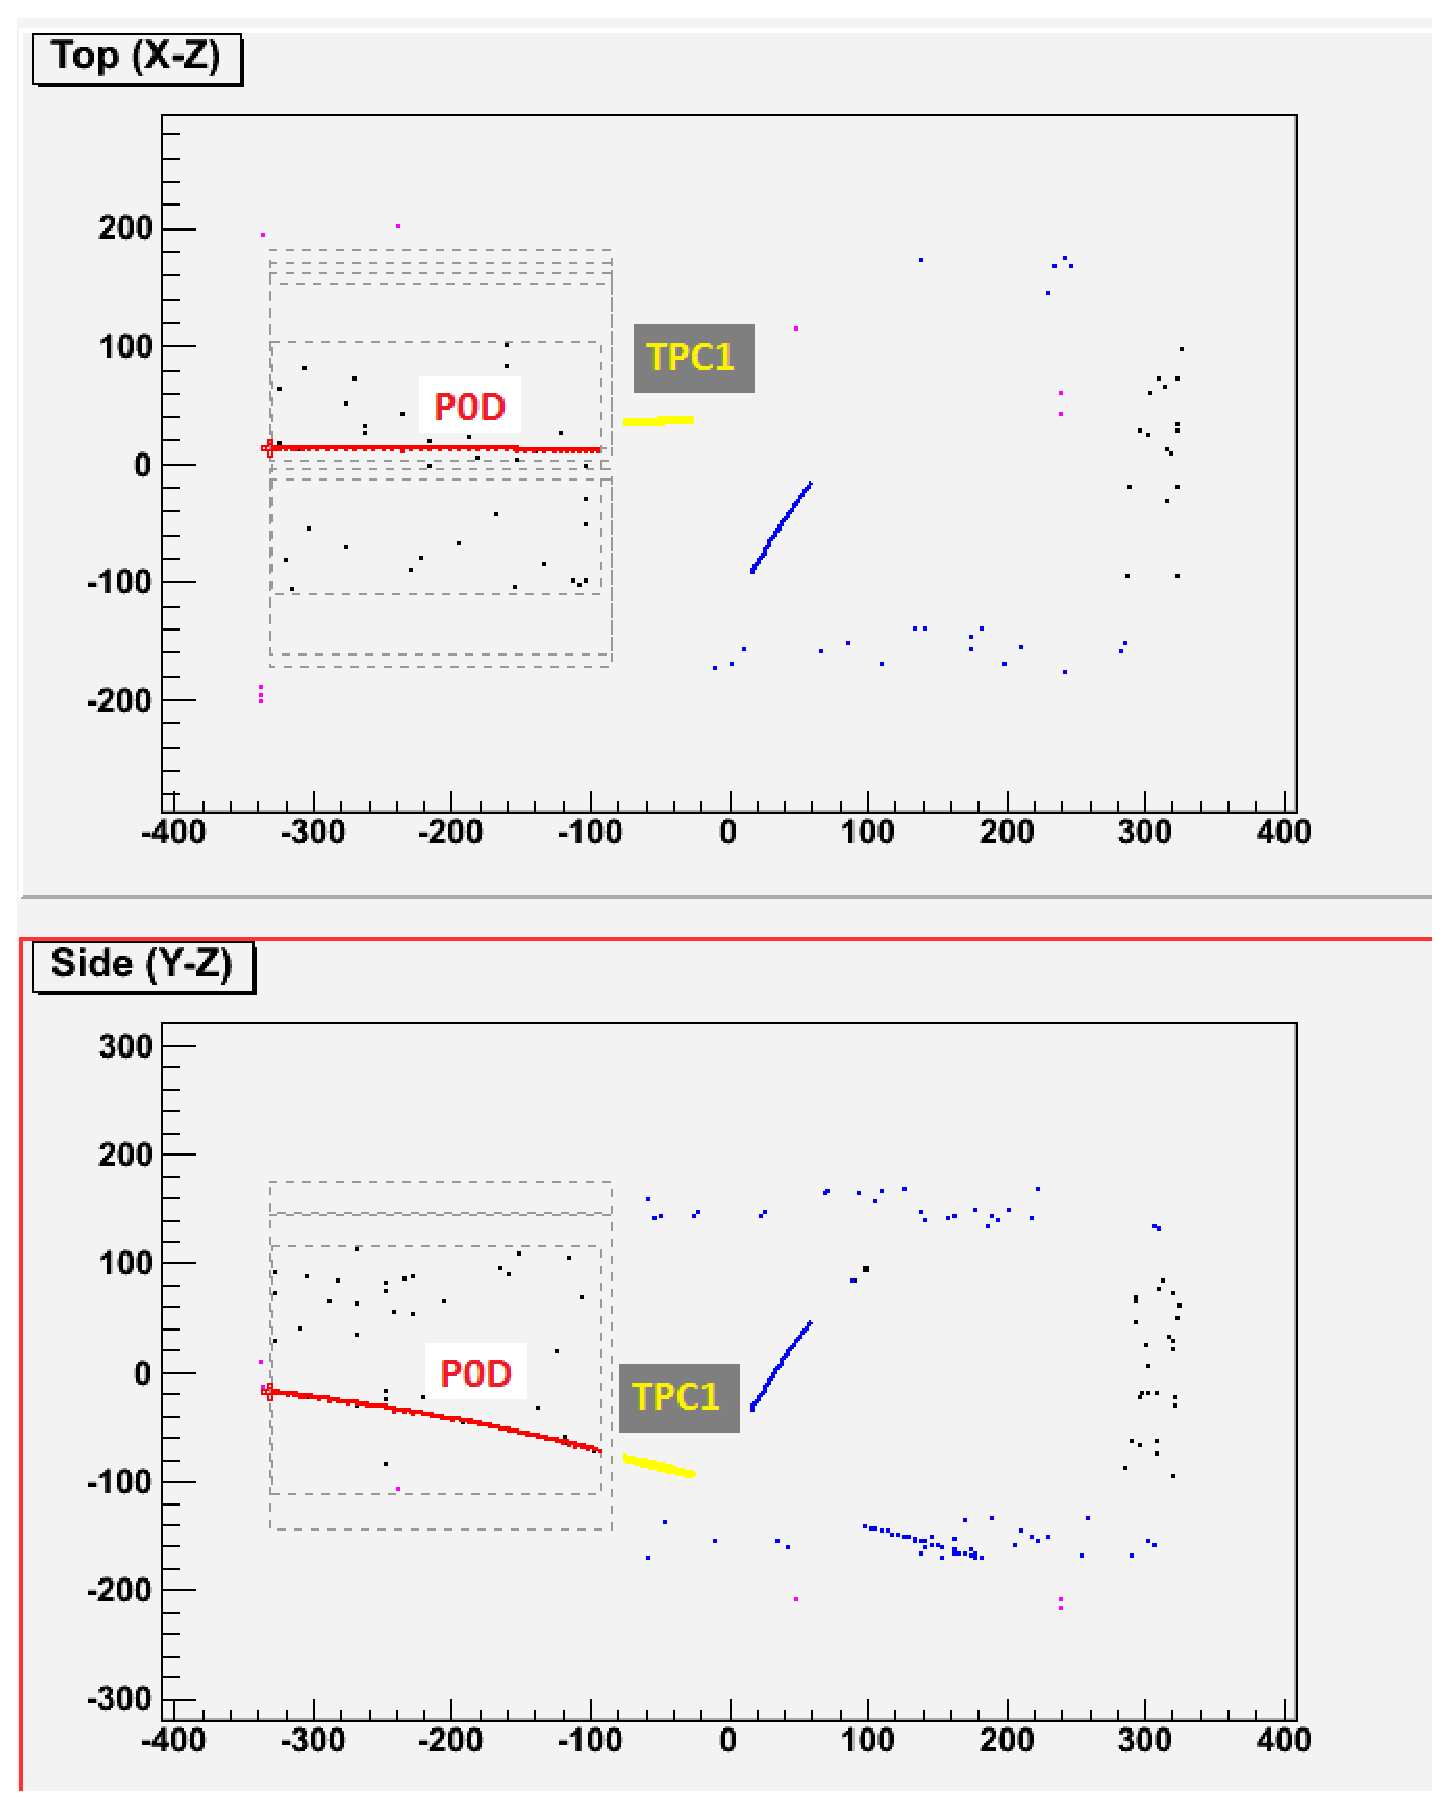
\includegraphics[width=3in]{Figures/t0mismatch.eps}
  \caption{An example of the $\Delta T$ (left) and $T0$ (right) failure modes. In the  $\Delta T$ failure, the \p0d track (red) and the Tracker track (blue) match perfectly spatially, but are disjoint in time by $>100$ns. In the $T0$, the YZ projection has a good spatial match between the \p0d track (red) and Tracker track (yellow), but the drift direction shows a symptomatic offset.} 
  \label{fig:mismatchexamples}
\end{figure}

We hand scanned Data events corresponding to $1.056\times 10^{19}$POT and MC events corresponding to $3.34\times 10^{18}$POT. The two timing related failure modes, $T0$ and $\Delta T$, were only observed in Data and never in MC. Closer examination of the failed events showed that though some were muon-like tracks originating inside the \p0d, many were actually sand muon events which made it through the veto. As the timing of the TPC1 track piece and the \p0d track piece were generally different in these events, our sand muon veto did not associate the hits in the outer edges of the \p0d with the TPC1 track, causing the sand muons to leak through our selection cuts. In Table \ref{tab:handscan} we summarize the number of events in Data that failed via the $T0$ and $\Delta T$ modes and whether they originated from inside or outside the \p0d.
\begin{table}[here]
\centering
\begin{tabular}{lcc}\toprule
& $\Delta T$ Failures & $T0$ Failures\\\midrule
Sand Muon & 11 & 20 \\
In-\p0d Muon & 10 & 9 \\\bottomrule
\end{tabular}
\caption{
Total number of events from the $\Delta T$ and $T0$ failure modes for sand muons and in-\p0d muon-like events.
}
\label{tab:handscan}
\end{table}

An examination of the $\Delta T$ failures show that none of the tracks have FGD constitutents. As the two control samples are predominantly tracks that pass through the FGD, the $\Delta T$ failure is most likely not accounted for in the efficiencies evaluated using Sand Muons and FGD Cosmics. We use the 10 $\Delta T$ In-\p0d failures as uncertainty in the Data event rate. 
Sand muon events which made it past our veto in this study would still be correctly rejected in the actual CC inclusive selection by the fiducial volume cut. However, the T0 effect is not necessarily replicated correctly in the cosmics and sand muon samples. When relatively steep tracks pass through TPC1 without also entering an FGD, the T0 is more likely to be miscalculated. Since FGD cosmics require the tracks to pass through the FGDs and sand muons are generally lengthy tracks passing through the entire ND280, T0 problems are less likely observed. So the hand scan study also adds a matching uncertainty due to the 9 muon-like tracks corresponding to the T0 failure mode. Also, even though the study was conducted on Production 4, we expect the errors to persist in Production 5 as the effect stems from tracks lacking FGD constituents.

Including the statistical errors appropriately, we have $19\pm 4.36$(stat.) events more in the Data from the T0 failure and the In-\p0d $\Delta T$ failure modes combined. When normalized to the total Data POT for each run type from the inclusive analysis, we get $422.28 \pm 96.88$  events per $23.47\times 10^{19}$POT for water-in running and $591.77 \pm 135.76$  events per $32.89\times 10^{19}$POT for water-out running.

\subsubsection{Results of Matching Efficiency Systematic Studies}
\label{sec:Systematics_MatchingEfficiencyResults}

From the FGD cosmic sample, the MC / Data efficiency ratio is $(99.22\%\pm 0.24\%) / (99.08\%\pm 0.16\%) = 100.14\%\pm 0.24\%$. This is the value we need to multiply the final Data to MC ratio by to correct for efficiency. Similarly, using the results from the hand-scanning procedure, we calculate corresponding correction factors of $1.017 \pm 0.0039$ for water-in and $1.023 \pm 0.0053$ for water-out. These correction factors are multiplicative and uncorrelated with the cosmics efficiency correction. Propagating errors in quadrature yields total correction factors of $1.018 \pm 0.0049$ for water-in and $1.024 \pm 0.0060$ for water-out. The Data to MC ratios are shifted by using this final correction factor. The corresponding errors are then $\pm 0.49 \%$ for water-in runs and $0.6 \%$ for water-out runs.

%Linearly adding and subtracting the error and the central value, we get the efficiency ratio ranges of 99.18\% to 99.92\% from cosmics and 99.83\% to 100.36\% from sand muons. Taking the widest possible limits, we get the range 99.18\% to 100.36\%. To this range, we add the results from the hand scanning study. Missing events in Data only adds to the efficiency systematic number. 
%So taking the lower and upper limits of the hand scanning result, we get a $(62-21) / 7845 = 0.0052$ shift in the lower limit of the efficiency systematic and a $(62+99) / 7845 = .0205$ shift in the upper limit. The adjusted lower and upper limits are then $0.9918 + 0.0052 = 0.997$ and $1.0036+0.0205 = 1.0241$ respectively. This yields a total systematic uncertainty of -0.3\% and +2.4\% from the various efficiency studies for Run 1 + Run 2.

% The 62 events that were missed in Data due to the T0 value corresponds to $62 / 7845 = 0.79\%$ of the total selected CC inclusive events. Missing events in Data adds to the upper limit of the efficiency systematic. So adding linearly again, we have the final efficiency ratio range of 99.18\% to 101.15\%. This corresponds to a systematic uncertainty of -0.82\% and +1.15\% from the various efficiency studies for Run 1 + Run 2.
